
% RADAR: Mitigating Byzantine Contributions in Heterogeneous Settings
% ------------------------------------------------------------------------------
\setlength{\titleoffset}{-1.05cm}
\section
  [{\texttt{RADAR}~\circled[contrib/radar]{R}}]
  {\circled[contrib/radar]{R}~Fighting Byzantine Contributions in Heterogeneous Settings}

% \begingroup
% \setbeamertemplate{frame footer}{\circled[contrib/radar]{R}~\texttt{RADAR}}

\begin{frame}[plain]
  \sectionpage

  \fcitefootnote{lavaur_radar_2024}
\end{frame}


\begin{frame}{Context}
  % - case study (multiple organizations, partial heterogeneity)
  % - Byzantine contributions -> no guaranties
  \textbf{Case study reminder}
  \begin{itemize}
    \item Multiple organizations collaborating on a federated Intrusion Detection System.
    \item Partial heterogeneity in the datasets: different data distributions but existing similarities.
  \end{itemize}

  \pause
  \textbf{Byzantine contributions:}
  \begin{itemize}
    %\item No guarantees on the quality of the contributions.
    %\item Can be intentional, due to poor data quality, or due to data distribution mismatches.
    \item data quality issues (\eg, labelling, noise);
    \item distribution mismatches; and
    \item adversaries, \textit{possibly colluding}.

  \end{itemize}

\end{frame}

\begin{frame}{Problem Statement}
  \begin{block}{Quality Assessment in Heterogeneous Settings}
    For $n$ participants $p_i$ and their local datasets $d_i$ of unknown similarity, each participant uploads a model update $w_i^r$ at each round $r$. Given $P = \{ p_1, p_2, \dots, p_n \} $ and $W = \{ w_1^r, w_2^r, \dots, w_n^r \} $, how can one assess the quality of each participant’s contribution without making assumptions on the data distribution across the datasets $d_i$?
  \end{block}
\end{frame}


\begingroup  % Remove the Author for this slide, as the citations step on the footer.
\setbeamertemplate{frame footer}{}
\begin{frame}{Existing Solutions}

  \begin{columns}[T]
    
    \begin{column}{.33\textwidth}
      \small\centering
      \textbf{Server-side evaluation}~\autocite{zhou_DifferentiallyPrivateFederated_2022}

      \begin{figure}
        \centering
        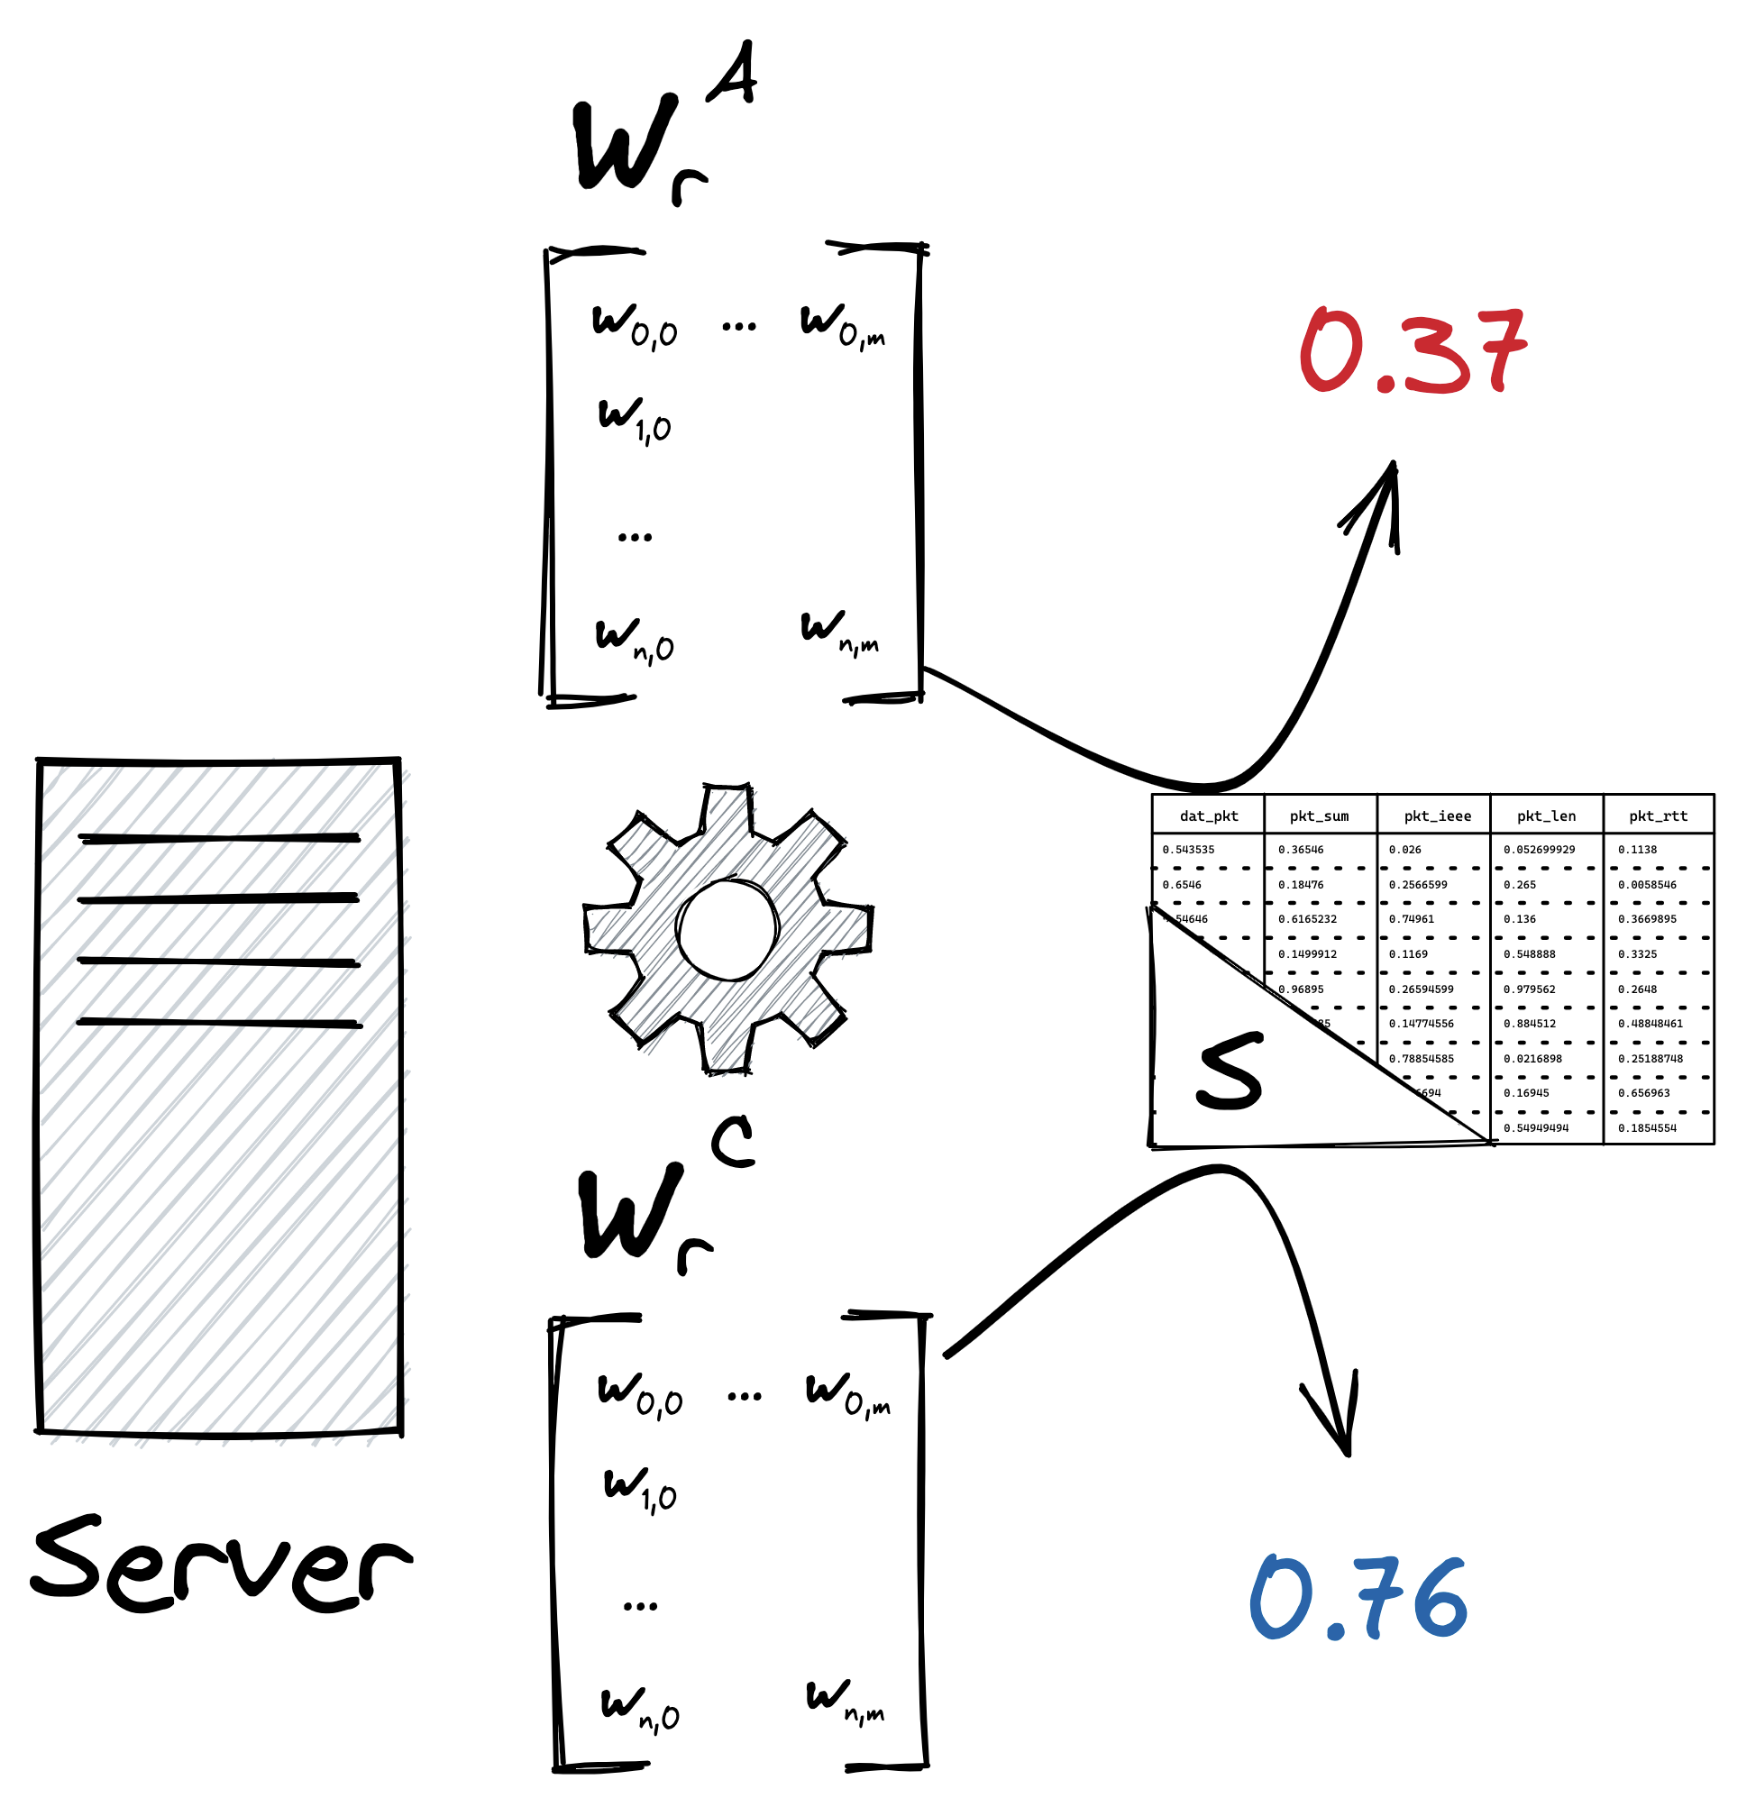
\includegraphics[height=.36\textheight]{figures/radar/server-side-eval}
      \end{figure}

      \begin{itemize}\smaller
        \item Only applicable in IID settings.
        \item Single source of truth.
      \end{itemize}
    \end{column}

    \onslide<2->{%
      \begin{column}{.33\textwidth}
        \small\centering
        \textbf{Server-side comparison}~\autocite{briggs_Federatedlearninghierarchical_2020}

        \begin{figure}
          \centering
          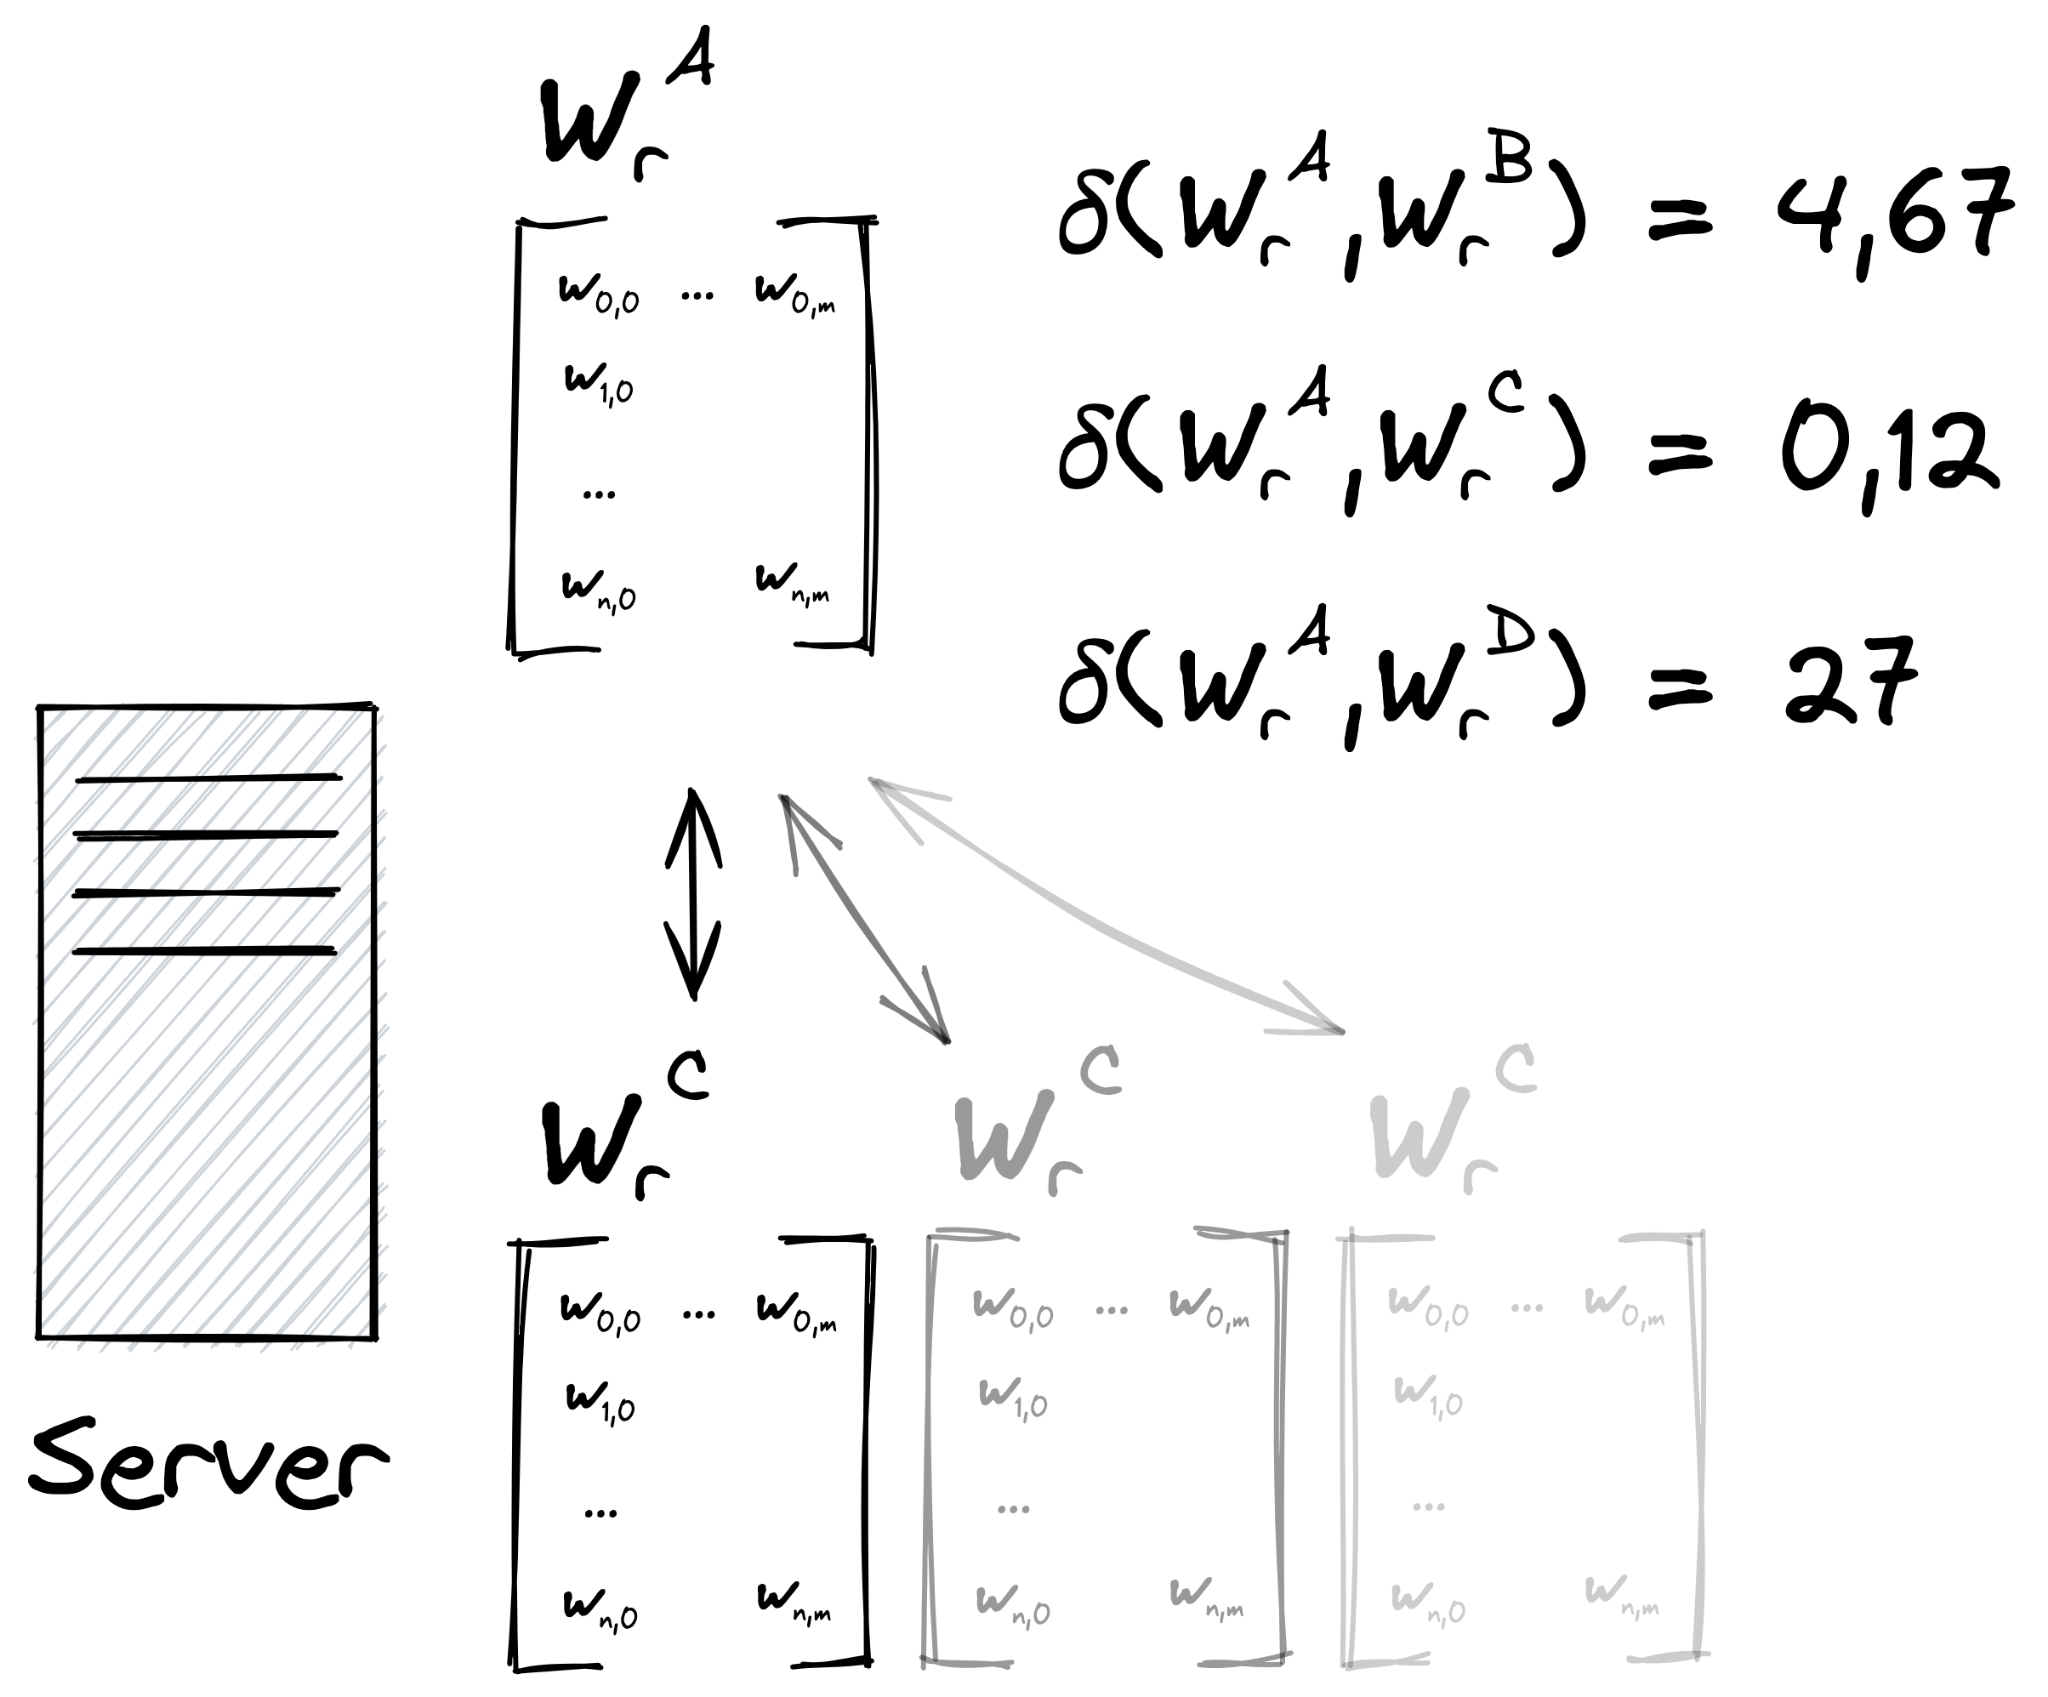
\includegraphics[height=.36\textheight]{figures/radar/server-side-comp}
        \end{figure}

        \begin{itemize}\smaller
          \item Less related to client data.
          %\item More appropriate for high-dimensional data.
        \end{itemize}
      \end{column}%
    }

    \onslide<3->{%
      \begin{column}{.33\textwidth}
        \small\centering
        \textbf{Client-side evaluation}~\autocite{zhao_ShieldingCollaborativeLearning_2020}

        \begin{figure}
          \centering
          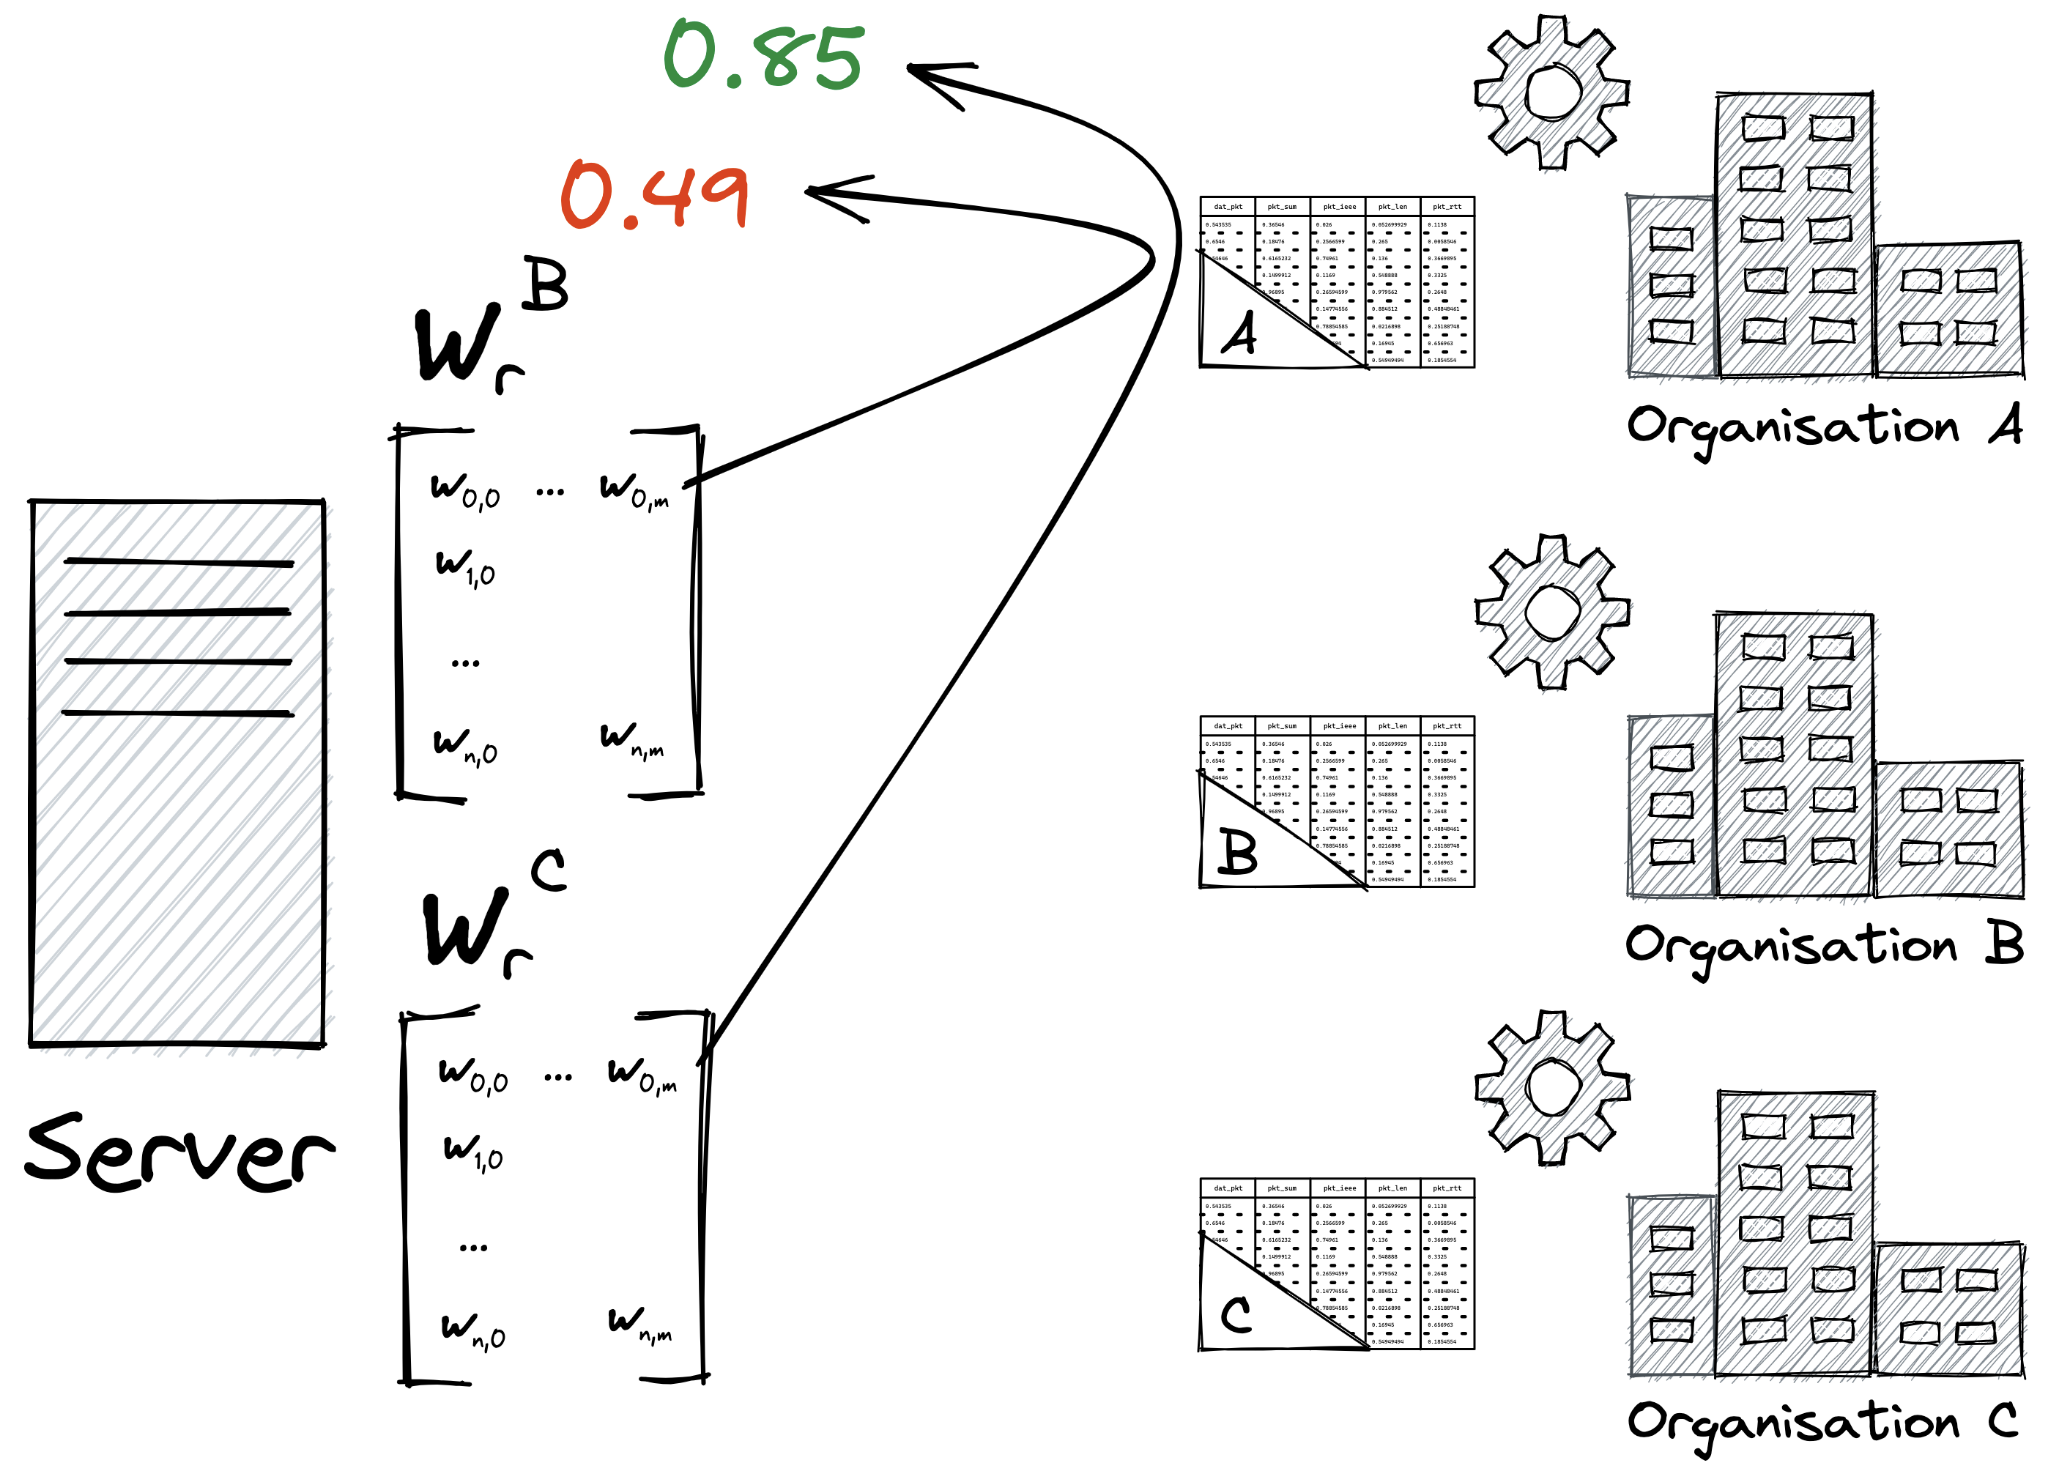
\includegraphics[height=.36\textheight]{figures/radar/client-side-eval}
        \end{figure}

        \begin{itemize}\smaller
          \item High cost in cross-device.
          \item More susceptible to badmouthing.
        \end{itemize}
      \end{column}%
    }

  \end{columns}

  \vspace{3ex}
  
  \fcitefootnote{zhou_DifferentiallyPrivateFederated_2022}
  \only<1>{\blankfootnote{}\blankfootnote{}\blankfootnote{}} % To keep the same height for the footnotes.
  \only<2->{\fcitefootnote{briggs_Federatedlearninghierarchical_2020}}
  \only<2>{\blankfootnote{}}
  \only<3->{\fcitefootnote{zhao_ShieldingCollaborativeLearning_2020}}

\end{frame}
\endgroup

\begin{frame}{Introducing \texttt{RADAR}}
  \centering
    \begin{figure}
        \centering
        \foreach \i in {1,...,4} {
          \includegraphics<\i>[width=.95\linewidth,left]{figures/radar/agenda/\i.pdf}%
        }
        \caption*{\texttt{RADAR} architecture. } % remove Figure:
        \label{fig:radar}
    \end{figure}  
         
    % \tableofcontents%[hideallsubsections,]
\end{frame}

\begin{frame}{Assessing Quality with Cross-Evaluation}

  \begin{columns}
    \begin{column}{.45\textwidth}
      \begin{figure}
        \centering
        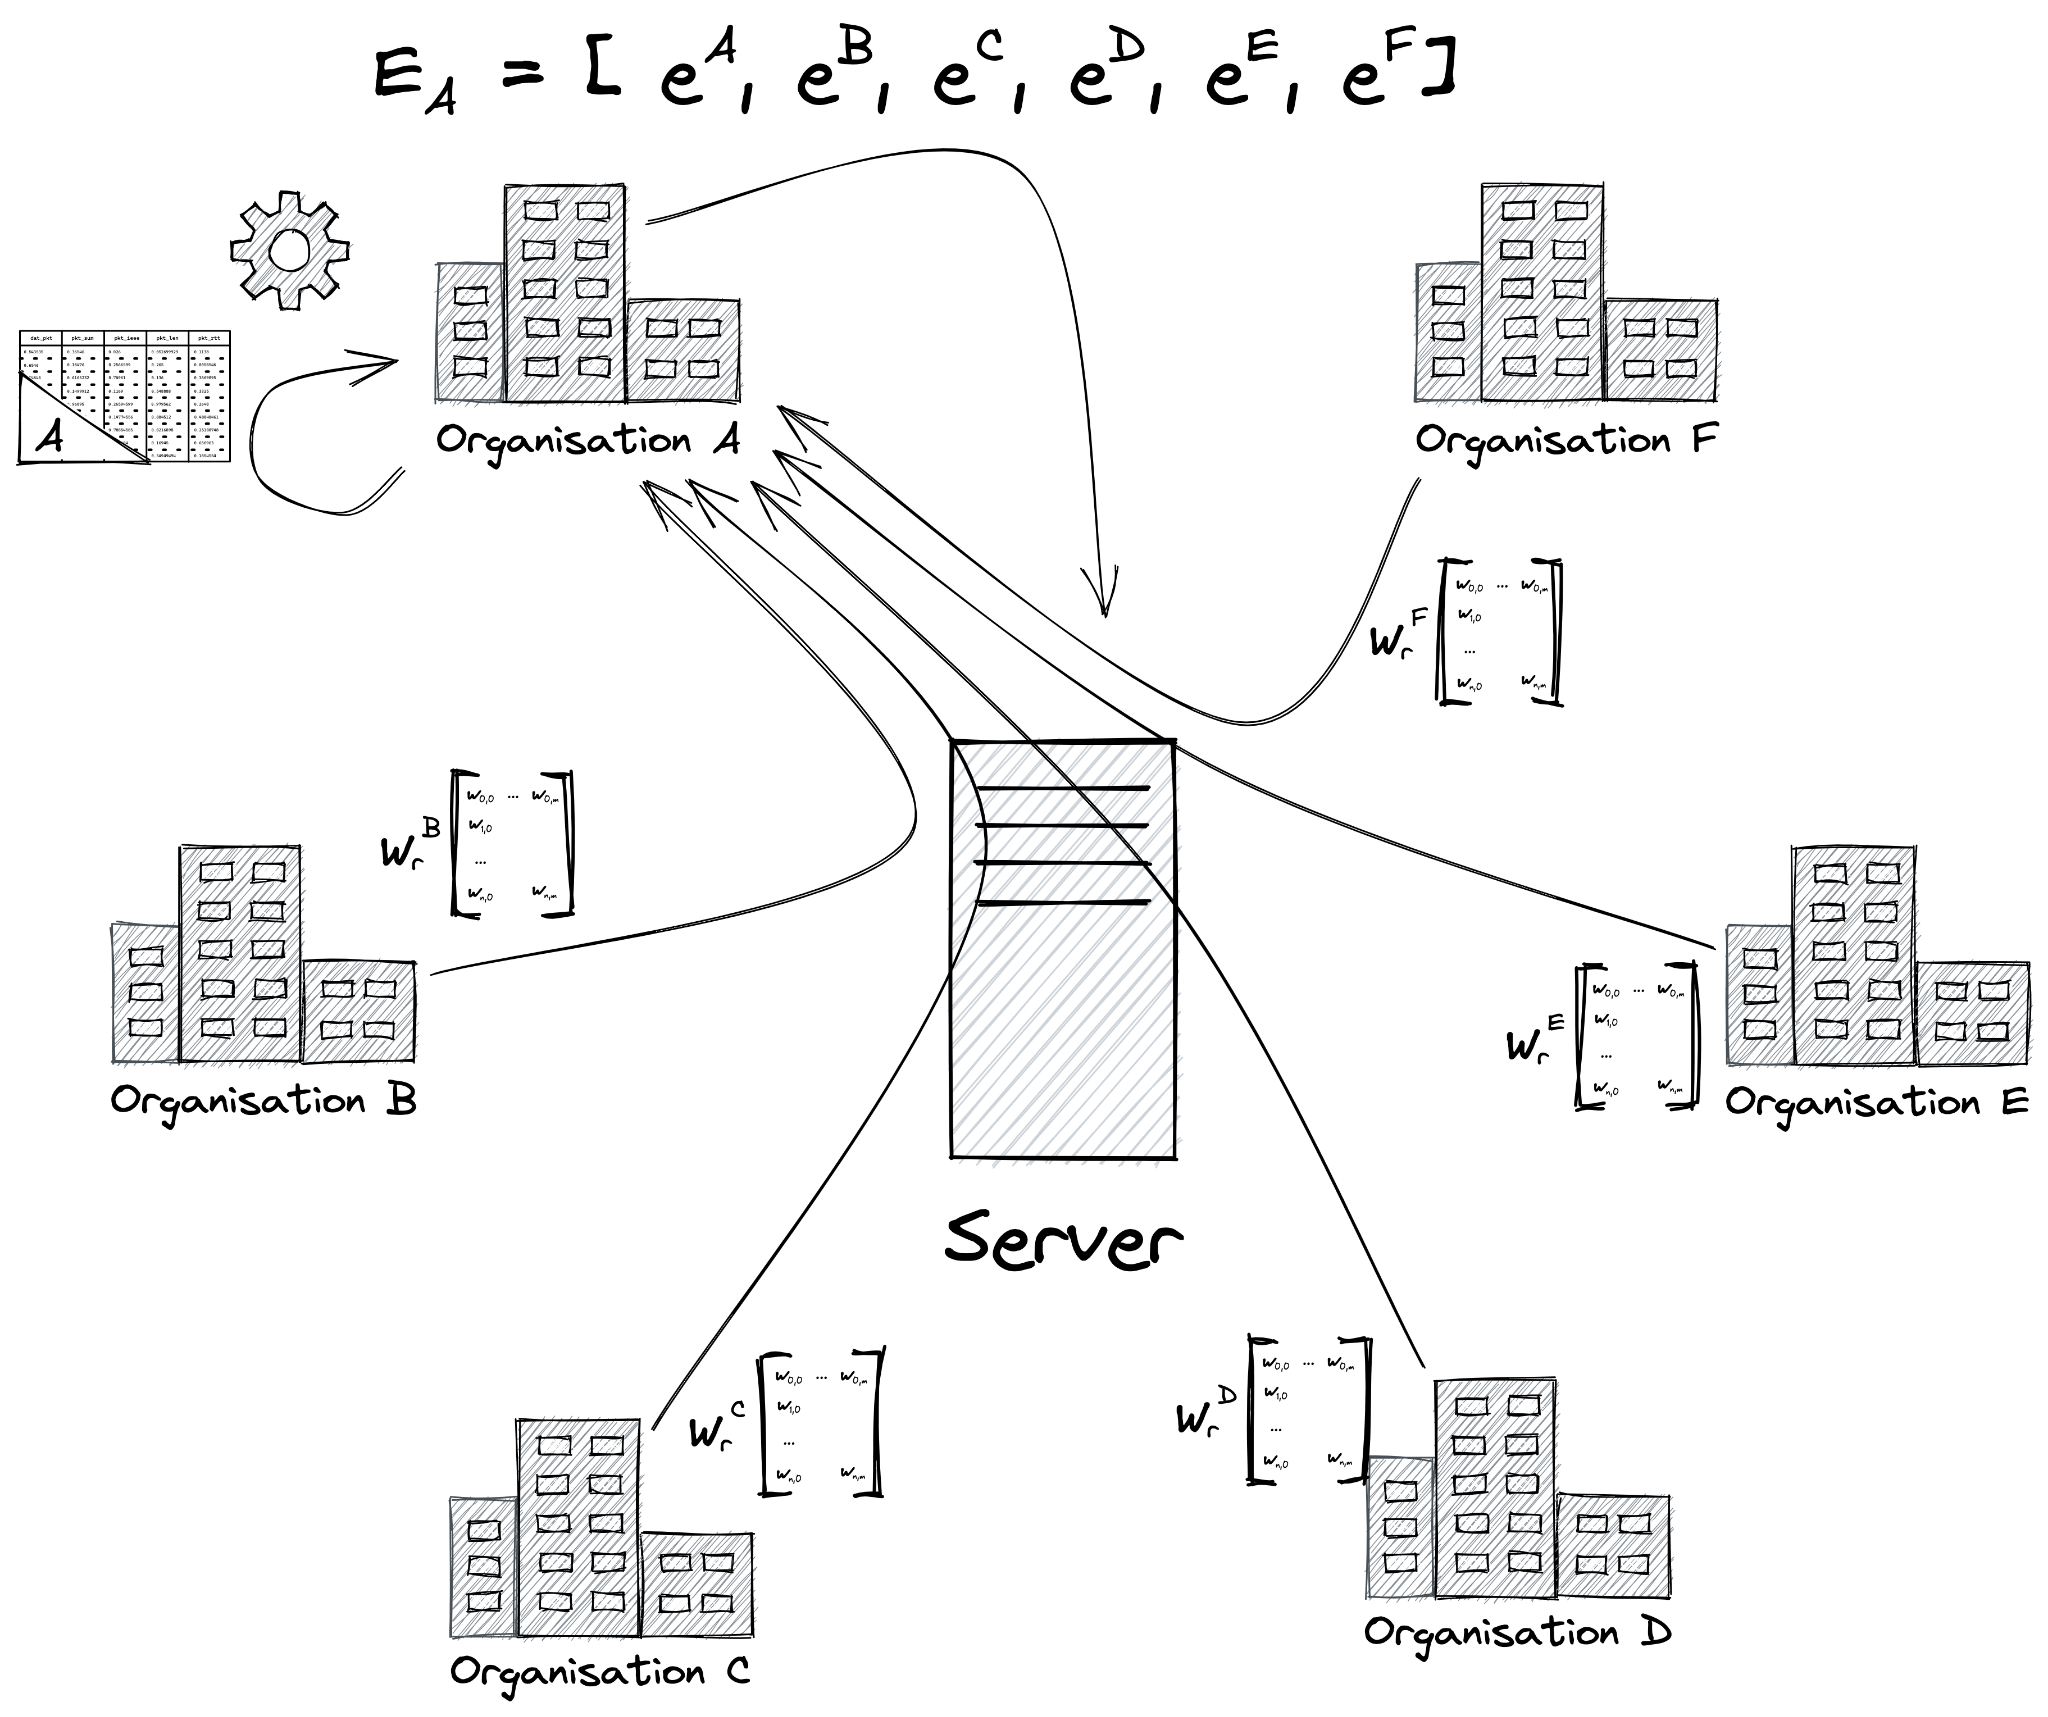
\includegraphics[width=\textwidth]{figures/radar/xeval}
      \end{figure}
    \end{column}
    
    \begin{column}{.55\textwidth}
      \small
      \setlength{\baselineskip}{0.8\baselineskip}
      \vspace{1ex}

      \textbf{Advantages}
      \begin{itemize}
        \item Exhaustive overview of the entire system at each round $r$. \alert{No need of prior knowledge!}
        \item Evaluations (\eg, accuracy, F1 score) representative of participants' data.
      \end{itemize}
      \medskip
      \pause
      \textbf{Drawbacks}
      \begin{itemize}
        \item High communication and computation costs.
        \item Does not scale well.
        %\item Shares local models to participants: less privacy-friendly.
      \end{itemize}
      \medskip
      \pause
      \textbf{But\dots}
      \begin{itemize}
        \item Cross-silo use case: few clients, with reasonable computing capacity.
        \item Slow workflow: long time between rounds.
      \end{itemize}
    \end{column}

  \end{columns}

\end{frame}



\begin{frame}{Fighting Heterogeneity with Clustering}
  \bigskip\bigskip
  \centering
  \begin{minipage}{.8\textwidth}
    \textbf{Objective}
    \begin{itemize}
      \item Build \emph{more} homogeneous communities of participants to facilitate model aggregation.
    \end{itemize}    
  \end{minipage}

  
  \begin{columns}
    \begin{column}{.5\textwidth}
      \pause
      \begin{itemize}
        \item Distance metric
        \begin{itemize}
            \item Based on \alert{cross-evaluation} results. 
            \item \alert{Cosine similarity}~\autocite{briggs_Federatedlearninghierarchical_2020}.
        \end{itemize}
      \end{itemize}
      
      \pause
      \begin{itemize}
        \item Algorithm
        \begin{itemize}
          \item \alert{Hierarchical clustering}.~\autocite{briggs_Federatedlearninghierarchical_2020}
          \item Dynamic aggregation threshold. 
        \end{itemize}
      \end{itemize}
    \end{column}


      \begin{column}{.5\textwidth}
        \begin{figure}
          \centering
          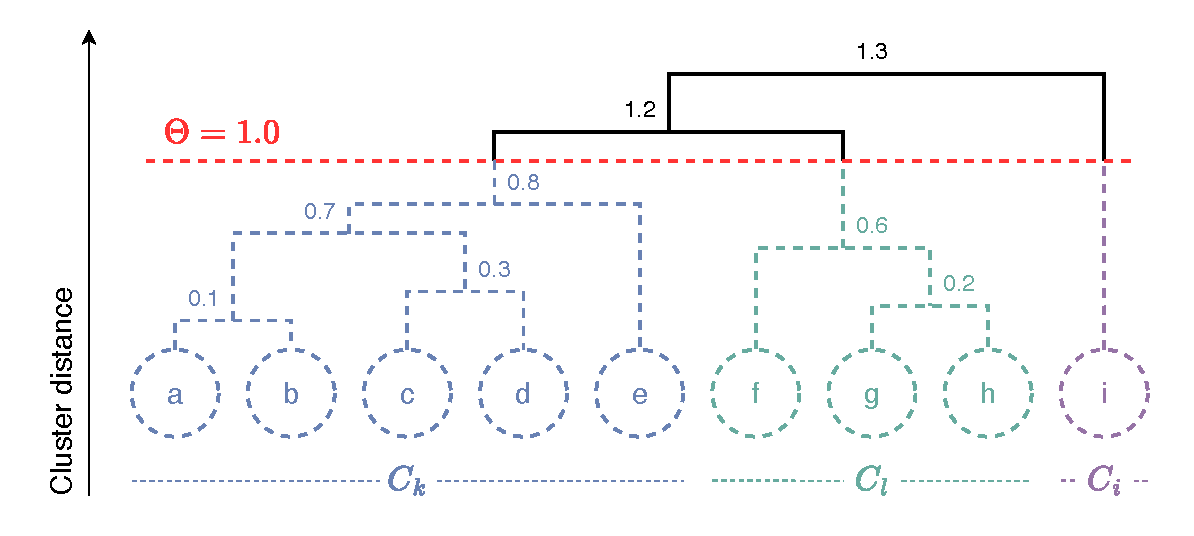
\includegraphics[width=\textwidth]{figures/radar/clustering.drawio.pdf}
          \caption{Hierarchical clustering.}
        \end{figure}
      \end{column}
  \end{columns}
  \bigskip
  \only<2->{\fcitefootnote{briggs_Federatedlearninghierarchical_2020}}

\end{frame}

% \begin{frame}{Fighting Heterogeneity with Clustering}
  
%   \textbf{Objective}
%   \begin{itemize}
%     \item Build \emph{more} homogeneous communities of participants to facilitate model aggregation.
%   \end{itemize}


%     \pause
%     \textbf{Clustering for FL}

%     \begin{columns}
        
%         \begin{column}{.5\textwidth}
%             \begin{itemize}
%                 \item Distance metric:
%                 \begin{itemize}
%                     \item Between models/gradients;
%                     \item L1/L2 Norm, cosine similarity\dots~\cite{briggs_Federatedlearninghierarchical_2020}
%                 \end{itemize}
%             \end{itemize}
%         \end{column}
    
%         \pause
%         \begin{column}{.45\textwidth}
%               \begin{itemize}
    
%               \item Algorithms:
%               \begin{itemize}
%                 \item Dynamic \emph{split-and-merge}.~\autocite{chen_ZeroKnowledgeClustering_2021}
%                 \item Hierarchical clustering.~\autocite{briggs_Federatedlearninghierarchical_2020}
%               \end{itemize}
%             \end{itemize}
    
%         \end{column}
%     \end{columns}

%     \only<2->{\fcitefootnote{briggs_Federatedlearninghierarchical_2020}}
%     \only<3->{\fcitefootnote{chen_ZeroKnowledgeClustering_2021}}
% \end{frame}

% \begin{frame}{Fighting Heterogeneity with Clustering}
%     \begin{columns}
%         \begin{column}{.4\textwidth}

%         Leverage cross-evaluation results instead of model updates:
%         \begin{itemize}
%             \item subjective similarity estimation;
%             \item similar evaluations $\rightarrow$ similar data distributions;
%         \end{itemize}

%         \end{column}
%         \begin{column}{.6\textwidth}
%             \begin{figure}
%                 \centering
%                 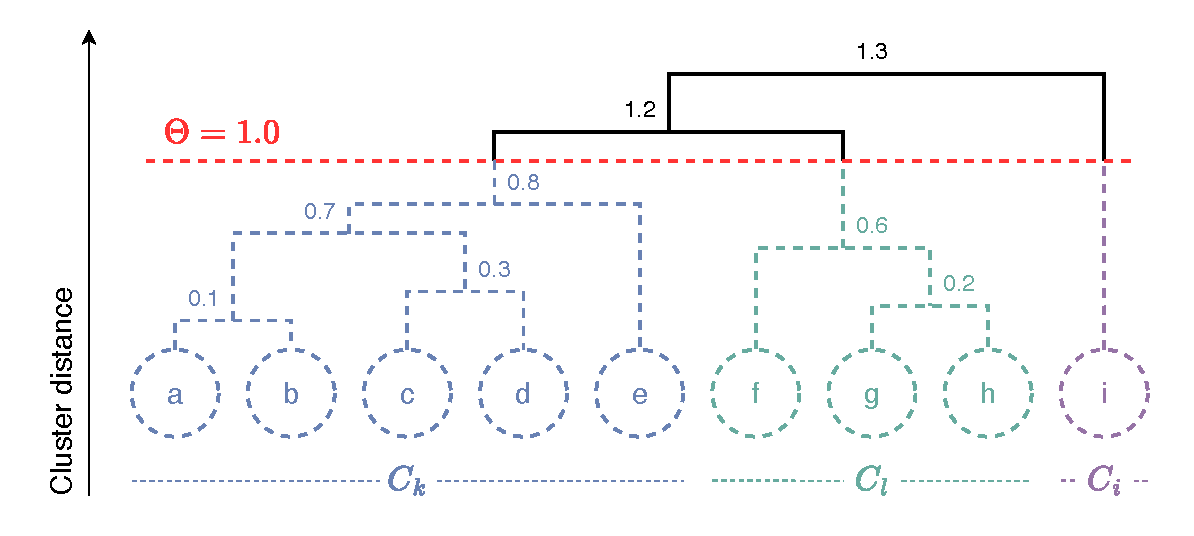
\includegraphics[width=\textwidth]{figures/radar/clustering.drawio.pdf}
%                 % \makebox[\textwidth][c]{%
%                 %   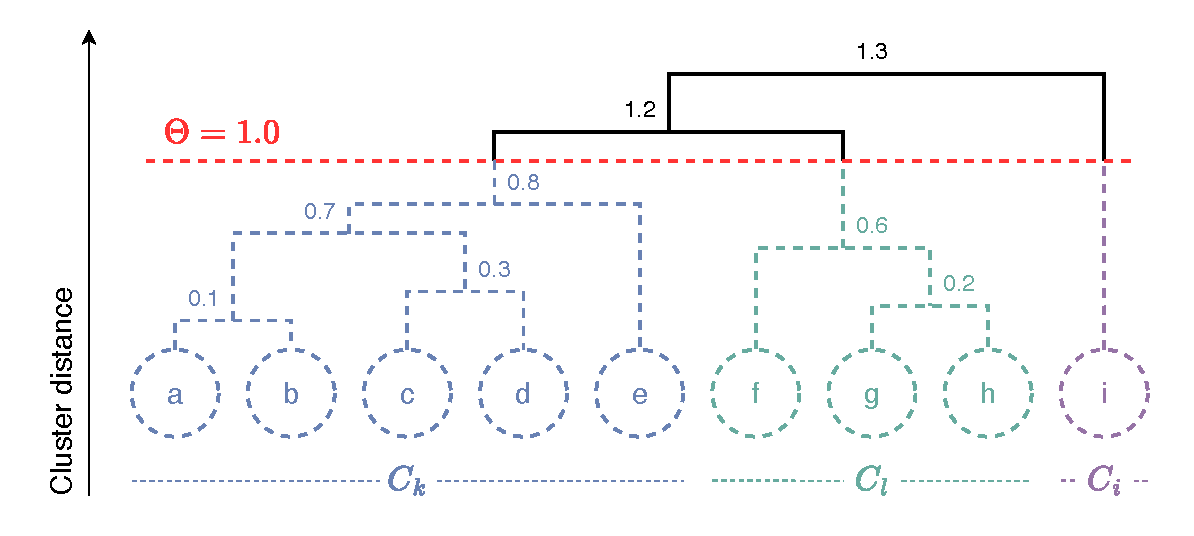
\includegraphics[width=1.2\textwidth]{figures/radar/clustering.drawio.pdf}%
%                 % }
%                 \caption{Hierarchical clustering.}
%             \end{figure}
%         \end{column}
%     \end{columns}
% \end{frame}


\begin{frame}{Reputation-aware Aggregation}

  \begin{block}{Definition: Reputation Systems\normalfont~\autocite{resnick_Reputationsystems_2000}}
    \begin{itemize}
      \item Long-lived entities expecting future interaction.
      \item Capture and distribution of feedback about current interactions (such information must be visible in the future).
      \item Use of feedback to guide trust decisions.
    \end{itemize}
  \end{block}
  \fcitefootnote{resnick_Reputationsystems_2000}

  \pause
  \begin{itemize}
    %\item Dirichlet distribution for local aggregation of the reputation scores.~\autocite{fung_DirichletBasedTrustManagement_2011}
    \item Votes weighted by the similarity inside each cluster.
    \item Exponential decay for potential redemption.
  \end{itemize}

\end{frame}

\begin{frame}{Setup: Simulating Practical Heterogeneity}

    \begin{columns}
      \begin{column}{.4\textwidth}
        \textbf{Datasets}
        \begin{itemize}
          \item Heterogeneous datasets, but some participants can share similarities.
          \item 4 datasets: CIC-CSE-IDS2018, UNSW-NB15, Bot-IoT, ToN\_IoT.
          \item NF-V2~\autocite{sarhan_StandardFeatureSet_2021} feature set (\ie, NetFlow V9).
        \end{itemize}
      \end{column}
      \begin{column}{.56\textwidth}
        \begin{figure}
          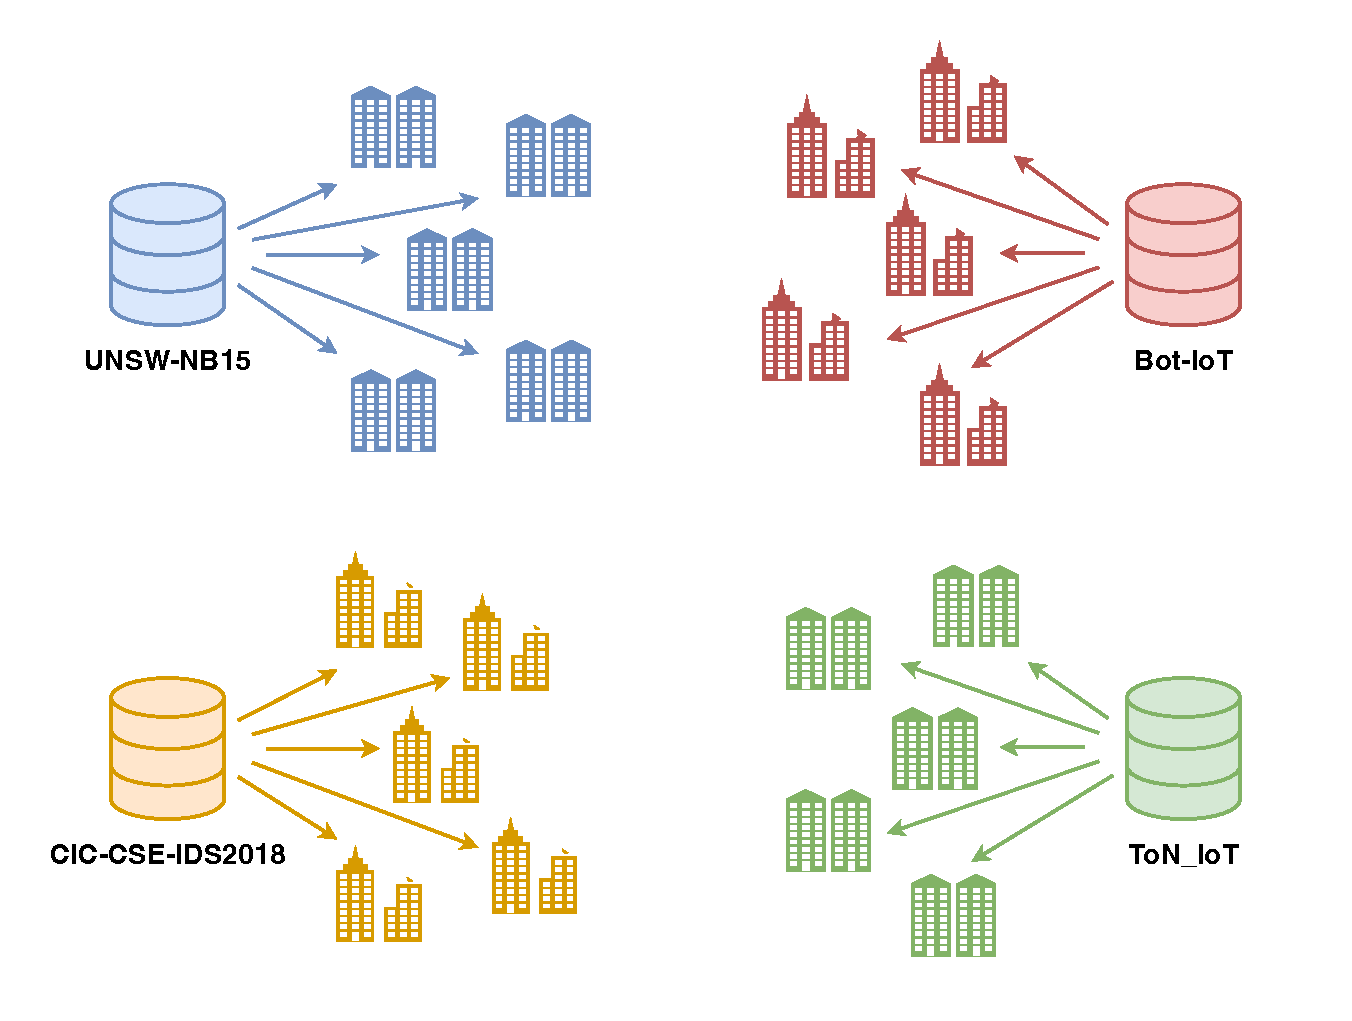
\includegraphics[width=\linewidth]{figures/radar/partition.pdf}%
        \end{figure}
      \end{column}
    \end{columns}
    \fcitefootnote{sarhan_StandardFeatureSet_2021}
  \end{frame}
  
  \begin{frame}{Setup: Byzantine Scenarios}
      \begin{columns}
          \begin{column}{.4\textwidth}
              \textbf{Parameters}
              \begin{itemize}
                  \item \textit{Target}: Affected classes.
                  \item \textit{Data Poisoning Rate (DPR)}: proportion of targeted data with flipped labels.
                  \item \textit{Model Poisoning Rate (MPR)}: number of attackers in the cluster.
              \end{itemize}
          \end{column}
          \begin{column}{.56\textwidth}
            \begin{figure}
              \captionsetup{font=small, labelfont=small}
              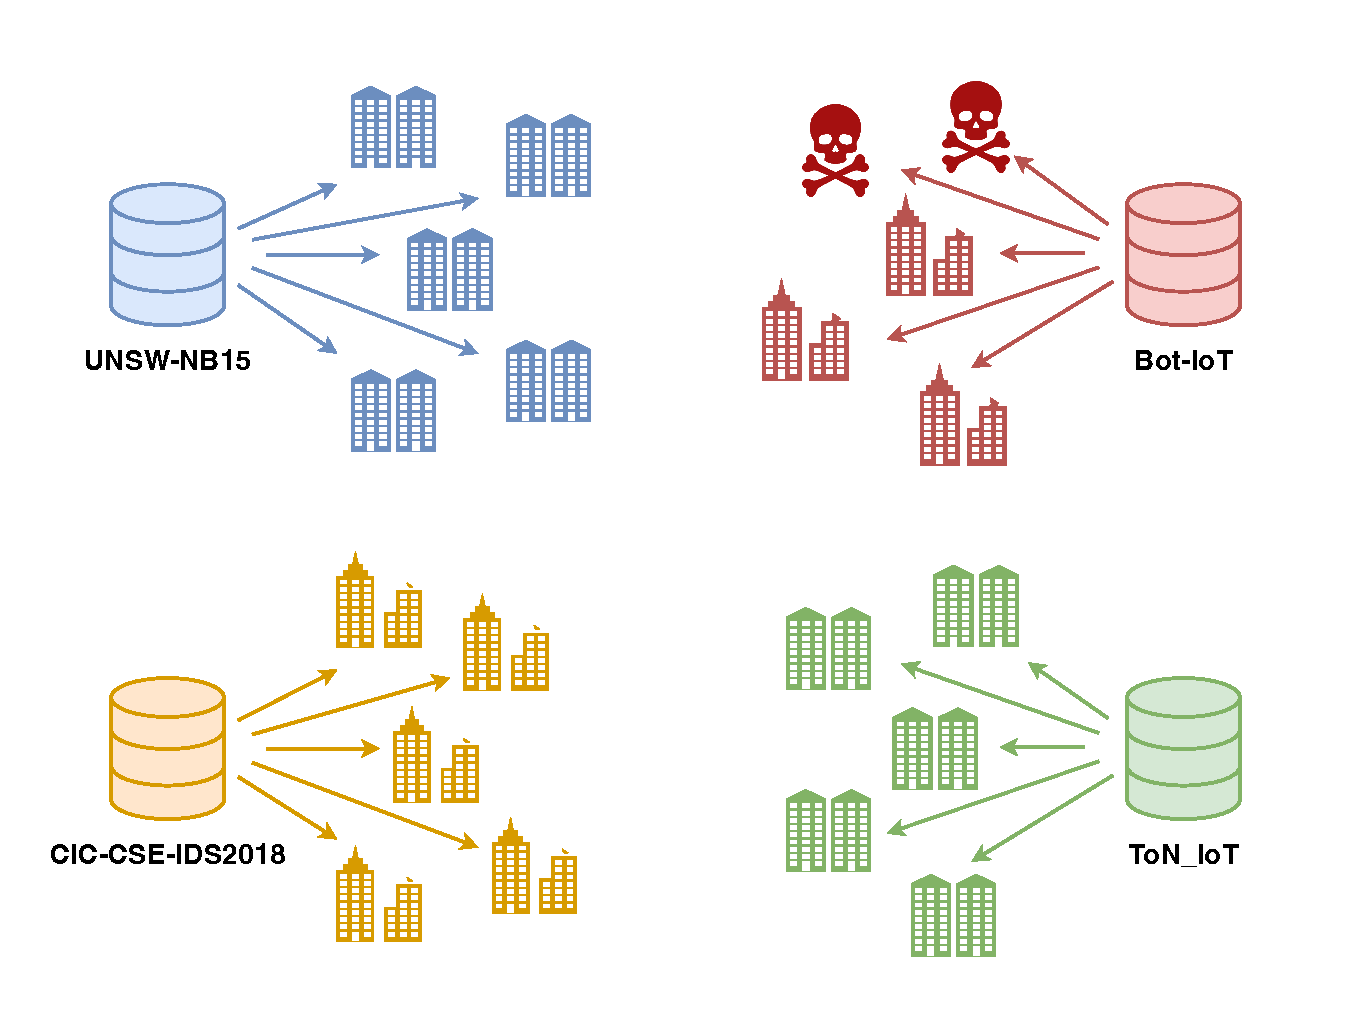
\includegraphics[width=\linewidth]{figures/radar/poisoning.pdf}%
              \captionsetup{justification=centering}
              \caption*{
                \texttt{colluding minority 100T}\\
                \smaller (\ie, 2 attackers, 100\% DPR on Reconnaissance class).
              }
            \end{figure}
          \end{column}
      \end{columns}
  \end{frame}

\begin{frame}{Results}
  \begin{table}
    \centering
    \caption{
      \emph{Effect of different attack configurations (untargeted) on all baselines.}
      \texttt{RA} is RADAR, \texttt{FG} is \texttt{FoolsGold}, \texttt{FA} is \texttt{FedAvg} (on \emph{all} participants), and \texttt{FC} is \texttt{FedAvg} ideally clustered per dataset.
    }

    \footnotesize

    \newcommand{\hl}{}
    \only<2>{\renewcommand{\hl}{\cellcolor{imta/green!30}}}


  
    \setlength\tabcolsep{1ex}
    \begin{tabularx}{.5\textwidth}{lX|rrrr}
      \toprule % ---------------------------------
      \multicolumn{2}{c|}{\multirow{2}{*}{\textbf{Scenario}}} & \multicolumn{4}{c}{\textbf{\gls{asr}} (\%)} \\
      & & \multicolumn{1}{c}{\texttt{RA}} & \multicolumn{1}{c}{\texttt{FG}} & \multicolumn{1}{c}{\texttt{FA}} & \multicolumn{1}{c}{\texttt{FC}} \\
      \midrule % ---------------------------------
      % TARGETED ATTACKS
      \multicolumn{2}{l|}{\textbf{Targeted} (\texttt{100T})} & & & & \\
                  & \hl \texttt{Benign}       &  \hl \textbf{0.00} &  5.17 & 5.10 &  0.09 \\
                  & \hl \texttt{Lone}         &  \hl \textbf{0.00} & 93.82 & 6.73 &  0.45 \\
                  & \hl \texttt{Collud. min.} &  \hl \textbf{0.00} &  2.97 & 9.99 & 53.40 \\
                  & \only<3>{\cellcolor{red!20}} \texttt{Collud. maj.} &  \only<3>{\cellcolor{red!20}} 73.39 & \textbf{8.10} & 17.65 & 59.36 \\
      \midrule % ---------------------------------
      % UNTARGETED ATTACKS
      \multicolumn{2}{l|}{\textbf{Untargeted} (\texttt{100U})} & & & & \\
      & \hl \texttt{Benign}        & \hl 0.09  & 0.39 & 33.30 & \textbf{0.06} \\
      & \hl \texttt{Lone}          & \hl \textbf{0.08} & 99.89 & 54.70 & 0.12 \\
      & \hl \texttt{Collud. min.}  & \hl 0.10 & \textbf{0.04} & 44.53 & 6.26 \\
      & \hl \texttt{Collud. maj.}  & \hl \textbf{0.08} & 38.98 & 59.49 & 94.36 \\          
      \bottomrule % ---------------------------------
      \small & \multicolumn{1}{c}{} & \multicolumn{4}{c}{\emph{lower is better}}
    \end{tabularx}
  \end{table}
  
\end{frame}

% \begin{frame}{Results}
%   \begin{figure}
%     \centering
%     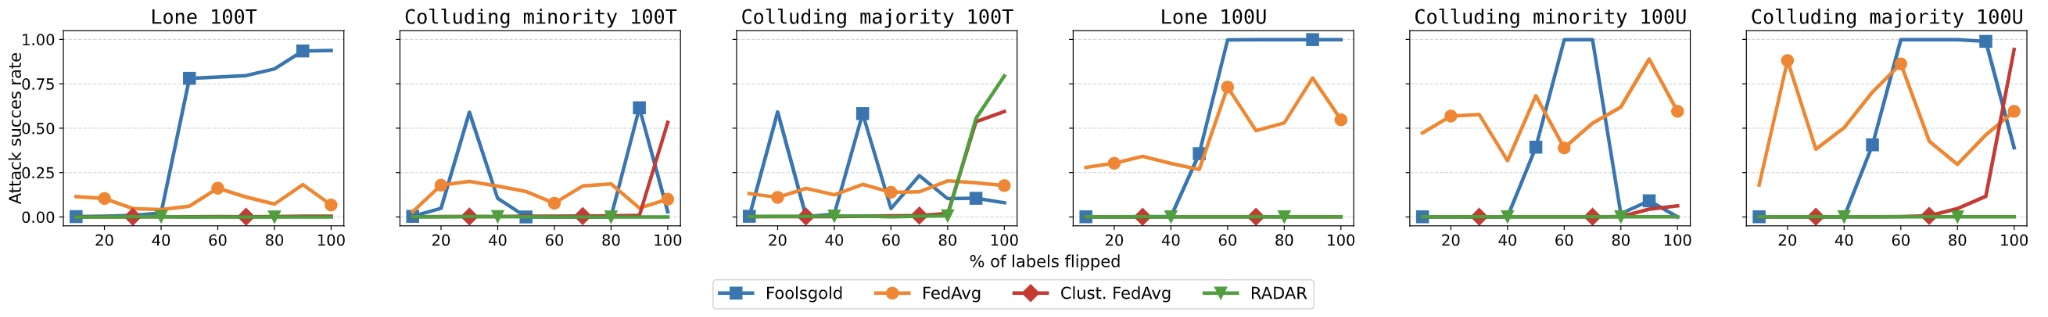
\includegraphics[width=.9\textwidth]{figures/radar/baselines.png}
%     \caption{Baseline comparison.}
%   \end{figure}
%   \begin{figure}
%     \centering
%     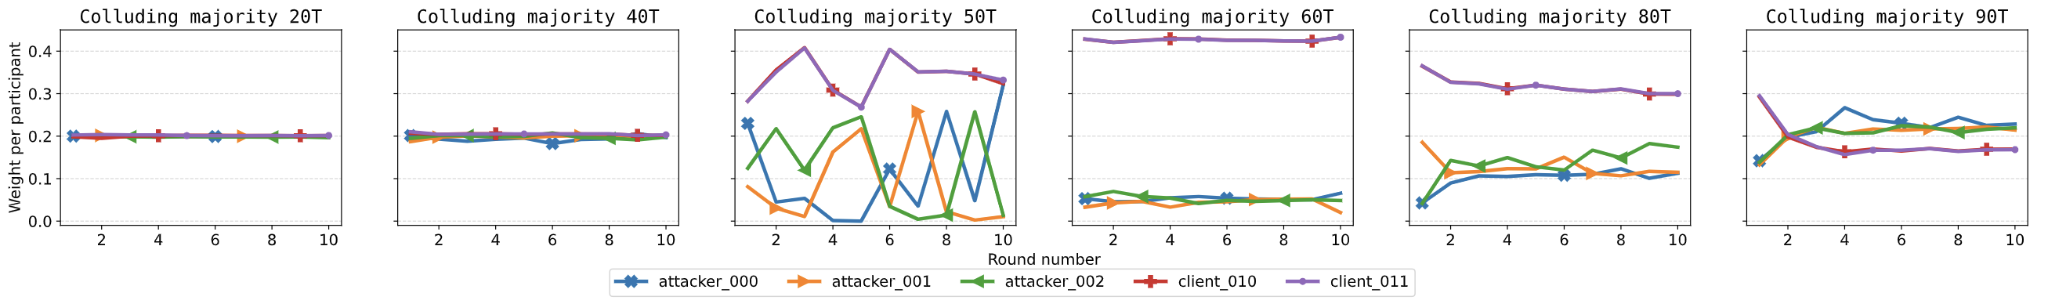
\includegraphics[width=.9\textwidth]{figures/radar/limiting-case.png}
%     \caption{RADAR's limiting scenario.}
%   \end{figure}
% \end{frame}

\begin{frame}{Takeways}
  \begin{enumerate}
    \onslide<+->
    \item \texttt{RADAR} can:
    \begin{itemize}
      \item leverage \alert{cross-evaluation}, \alert{clustering} and \alert{reputation} to address heterogeneity and Byzantine contributions;
      \item adjust rapidly to changes in behavior; and
      \item mitigate most tested scenarios (limiting case handled up to 80\% of poisoned data).
    \end{itemize}

    \medskip
    \onslide<+->
    \item How generic?
    \begin{itemize}
      \item Only few conditions: parametric models, locally owned evaluation set, a \alert<+->{small-scale use case}, and a \alert<.->{trusted central server}.
    \end{itemize}

    \medskip
    \onslide<+->
    \item Future works:
    \begin{itemize}
      \item Remove the central server dependency for \alert{increased trust and scalability}.
      \item Test the approach in more realistic heterogeneous settings.
    \end{itemize}
  \end{enumerate}
  


  % \pause
  % \textbf{How generic?}
  % \begin{itemize}
  %   \item Only few conditions: parametric models, locally owned evaluation set, a \alert<3>{small-scale use case}, and a \alert<3>{trusted central server}.
  % \end{itemize}

  % \pause
  % \textbf{Future works:}
  %   \begin{itemize}
  %     \item Remove the central server dependency for \alert{increased trust and scalability}.
  %     \item Test the approach in more realistic heterogeneous settings.
  %   \end{itemize}
\end{frame}